\documentclass[table]{beamer}
%[]中可以使用draft、handout、screen、transparency、trancompress、compress等参数

%指定beamer的模式与主题
\mode<presentation>
{
  \usetheme{Madrid}
%\usetheme{Boadilla}
%\usecolortheme{default}
%\usecolortheme{orchid}
%\usecolortheme{whale}
%\usefonttheme{professionalfonts}
}

%\usetheme{Madrid}
%这里还可以选择别的主题:Bergen, Boadilla, Madrid, AnnArbor, CambridgeUS, Pittsburgh, Rochester, Warsaw, ...
%有导航栏的Antibes, JuanLesPins, Montpellier, ...
%有内容的Berkeley, PaloAlto, Goettingen, Marburg, Hannover, ...
%有最小导航栏的Berlin, Ilmenau, Dresden, Darmstadt, Frankfurt, Singapore, Szeged, ...
%有章和节表单的Copenhagen, Luebeck, Malmoe, Warsaw, ...

%\usecolortheme{default}
%设置内部颜色主题(这些主题一般改变block里的颜色);这个主题一般选择动物来命名
%这里还可以选择别的颜色主题,如默认的和有特别目的的颜色主题default,structure,sidebartab,全颜色主题albatross,beetle,crane,dove,fly,seagull,wolverine,beaver

%\usecolortheme{orchid}
%设置外部颜色主题(这些主题一般改变title里的颜色);这个主题一般选择植物来命名
%这里还可以选择别的颜色主题,如默认的和有特别目的的颜色主题lily,orchid,rose

%\usecolortheme{whale}
%设置字体主题;这个主题一般选择海洋动物来命名
%这里还可以选择别的颜色主题,如默认的和有特别目的的颜色主题whale,seahorse,dolphin

%\usefonttheme{professionalfonts}
%类似的还可以定义structurebold,structuresmallcapsserif,professionalfonts

% 控制 beamer 的风格,可以根据自己的爱好修改
%\usepackage{beamerthemesplit} %使用 split 风格
%\usepackage{beamerthemeshadow} %使用 shadow 风格
%\usepackage[width=2cm,dark,tab]{beamerthemesidebar}

%插入音标
%\usepackage{tipa}
%\AtBeginDocument{
  %\renewcommand\textipa{\fontencoding{T3}\selectfont}
%}
%\AtBeginDocument{
  %\renewcommand\textipa[2][r]{{\fontfamily{cm#1}\tipaencoding #2}}
%}
%\renewenvironment{IPA}[1][r]
 %{\fontfamily{cm#1}\tipaencoding}
 %{}

% 设定英文字体
%\usepackage{fontspec}
% Fix bugs for fontspec in TeXLive2015
\ifdefined\suppressfontnotfounderror
  \expandafter\let\csname xetex_suppressfontnotfounderror:D\endcsname
    \suppressfontnotfounderror
\else
  \expandafter\let\csname xetex_suppressfontnotfounderror:D\endcsname
    \luatexsuppressfontnotfounderror
\fi
\usepackage[no-math]{fontspec}
\setmainfont{Times New Roman}
\setsansfont{Arial}
\setmonofont{Courier New}

% 设定中文字体
\usepackage[BoldFont,SlantFont,CJKchecksingle,CJKnumber]{xeCJK}
%\setCJKmainfont[BoldFont={Adobe Heiti Std},ItalicFont={Adobe Kaiti Std}]{Adobe Song Std}
\setCJKmainfont[BoldFont={Adobe Heiti Std},ItalicFont={Adobe Kaiti Std}]{WenQuanYi Micro Hei}
\setCJKsansfont{Adobe Heiti Std}
\setCJKmonofont{Adobe Fangsong Std}
\punctstyle{hangmobanjiao}

\defaultfontfeatures{Mapping=tex-text}
\usepackage{xunicode}
\usepackage{xltxtra}

\XeTeXlinebreaklocale "zh"
\XeTeXlinebreakskip = 0pt plus 1pt minus 0.1pt

\usepackage{setspace}
\usepackage{colortbl,xcolor}
\usepackage{hyperref}
%\hypersetup{xetex,bookmarksnumbered=true,bookmarksopen=true,pdfborder=1,breaklinks,colorlinks,linkcolor=blue,filecolor=black,urlcolor=cyan,citecolor=green}
\hypersetup{xetex,bookmarksnumbered=true,bookmarksopen=true,pdfborder=1,breaklinks,colorlinks,linkcolor=cyan,filecolor=black,urlcolor=blue,citecolor=green}

% 插入图片
\usepackage{graphicx}
\graphicspath{{figures/}}
% 图文混排
%\usepackage{picins}
\usepackage{floatflt}

% 可能用到的包
\usepackage{amsmath,amssymb}
%插入多媒体
%\usepackage{media9}
%\usepackage{movie15}
\usepackage{multimedia}
\usepackage{multicol}
\usepackage{multirow}

% 定义一些自选的模板,包括背景、图标、导航条和页脚等,修改要慎重
% 设置背景渐变由10%的红变成10%的结构颜色
%\beamertemplateshadingbackground{red!10}{structure!10}
%\beamertemplatesolidbackgroundcolor{white!90!blue}
% 使所有隐藏的文本完全透明、动态,而且动态的范围很小
\beamertemplatetransparentcovereddynamic
% 使itemize环境中变成小球,这是一种视觉效果
\beamertemplateballitem
% 为所有已编号的部分设置一个章节目录,并且编号显示成小球
\beamertemplatenumberedballsectiontoc
% 将每一页的要素的要素名设成加粗字体
\beamertemplateboldpartpage

% item逐步显示时,使已经出现的item、正在显示的item、将要出现的item呈现不同颜色
\def\hilite<#1>{
 \temporal<#1>{\color{gray}}{\color{blue}}
    {\color{blue!25}}
}

\renewcommand{\today}{\number\year 年 \number\month 月 \number\day 日}

%五角星
\usepackage{MnSymbol}

%去除图表标题中的figure等
\usepackage{caption}
\captionsetup{labelformat=empty,labelsep=none}

\usepackage{tabu}
\usepackage{multirow}
%表格自动换行
\usepackage{tabularx} 

% 千分号
%\usepackage{textcomp}

%罗马数字
\makeatletter
\newcommand{\rmnum}[1]{\romannumeral #1}
\newcommand{\Rmnum}[1]{\expandafter\@slowromancap\romannumeral #1@}
\makeatother

%分栏
\usepackage{multicol}

%\usepackage{enumitem}
%\usepackage{enumerate}

%键盘
\usepackage{keystroke}

%心形
\usepackage{fdsymbol}

%插入源代码
\usepackage{listings}
\lstset{
  language=perl,                  % 程序语言名称:TeX, Perl, R, sh, bash, Awk
  basicstyle=\normalsize\tt,      %\tt指monospace字体族,程序源代码使用此族字体表示更加美观
  numbers=left,                   % 行号位置(左侧)
  numberstyle=\small,             % 行号字体的字号
  stepnumber=1,                   % 行号的显示步长
  numbersep=5pt,                  % 行号与代码间距
  backgroundcolor=\color{white},  % 背景色;需要 \usepackage{color}
  showspaces=false,               % 不显示空格
  showstringspaces=false,         % 不显示代码字符串中的空格标记
  showtabs=false,                 % 不显示 TAB
  tabsize=4, 
  frame=shadowbox,                % 把代码用带有阴影的框圈起来
  captionpos=b,                   % 标题位置
  breaklines=true,                % 对过长的代码自动断行
  breakatwhitespace=false,        % 断行只在空格处
  extendedchars=false,            % 解决代码跨页时,章节标题,页眉等汉字不显示的问题
  %escapeinside={\%*}{*},         % 跳脱字符,添加注释,暂时离开 listings 
  %escapeinside=``,
  commentstyle=\color{red!50!green!50!blue!50}\tt,  %浅灰色的注释
  rulesepcolor=\color{red!20!green!20!blue!20},     %代码块边框为淡青色
  keywordstyle=\color{blue!70}\bfseries\tt,         %代码关键字的颜色为蓝色,粗体
  identifierstyle=\tt,
  stringstyle=\tt,                % 代码字符串的特殊格式
  keepspaces=true,
  breakindent=1em,
  %breakindent=22pt,
  %breakindent=4em,
  breakautoindent=true,
  flexiblecolumns=true,
  aboveskip=1em,                  %代码块边框
  xleftmargin=2em,
  xrightmargin=2em
}

%\setbeamercolor{alerted text}{fg=magenta}
\setbeamercolor{bgcolor}{fg=yellow,bg=cyan}
%\setbeamercolor{itemize/enumerate body}{fg=green}

\begin{document}

%\includeonlyframes{current}

\logo{\includegraphics[height=0.08\textwidth]{tijmu.png}}

% 在每个Section前都会加入的Frame
\AtBeginSection[]
{
  \begin{frame}<beamer>
    %\frametitle{Outline}
    \frametitle{教学提纲}
    \setcounter{tocdepth}{3}
    \begin{multicols}{2}
      \tableofcontents[currentsection,currentsubsection]
      %\tableofcontents[currentsection]
    \end{multicols}
  \end{frame}
}
% 在每个Subsection前都会加入的Frame
\AtBeginSubsection[]
{
  \begin{frame}<beamer>
%%\begin{frame}<handout:0>
%% handout:0 表示只在手稿中出现
    \frametitle{教学提纲}
    \setcounter{tocdepth}{3}
    \begin{multicols}{2}
    \tableofcontents[currentsection,currentsubsection]
    \end{multicols}
%% 显示在目录中加亮的当前章节
  \end{frame}
}

% 为当前幻灯片设置背景
%{
%\usebackgroundtemplate{
%\vbox to \paperheight{\vfil\hbox to
%\paperwidth{\hfil\includegraphics[width=2in]{tijmu_charcoal.png}\hfil}\vfil}
%}
\begin{frame}[plain]
  \begin{center}
    {\Huge 分子生物计算\\}
    {\huge \textit{(Perl语言编程)}\\}
    \vspace{1cm}
    {\LARGE 天津医科大学\\}
    %\vspace{0.2cm}
    {\LARGE 生物医学工程与技术学院\\}
    \vspace{1cm}
    {\large 2019-2020学年上学期(秋)\\ 2017级生信班}
  \end{center}
\end{frame}
%}



\title[限制酶图谱和正则表达式]{第九章\quad 限制酶图谱和正则表达式}
\author[Yixf]{伊现富(Yi Xianfu)}
\institute[TIJMU]{天津医科大学(TIJMU)\\ 生物医学工程与技术学院}
\date{2016年12月}

\input{snippet/beamer_toc.tex}

\section{引言}
\begin{frame}
  \frametitle{酶切图谱 | 引言}
  \begin{block}{已经学习}
    \begin{itemize}
      \item Perl语言
	\begin{itemize}
	  \item 正则表达式相关:模式匹配,字符替换
	  \item 操作符:数字操作符,字符串操作符
	\end{itemize}
      \item 生物信息学
	\begin{itemize}
	  \item 处理FASTA格式的文件
	  \item 在DNA序列中查找基序
	\end{itemize}
    \end{itemize}
  \end{block}
  \pause
  \begin{block}{即将学习}
    \begin{itemize}
      \item Perl语言
	\begin{itemize}
	  \item 正则表达式的基本理念
	  \item 操作符的优先级
	\end{itemize}
      \item 生物信息学
	\begin{itemize}
	  \item 用正则表达式表征酶切数据
	  \item 根据用户要求制作酶切图谱
	\end{itemize}
    \end{itemize}
  \end{block}
\end{frame}

\section{正则表达式}
\subsection{简介}
\begin{frame}[fragile]
  \frametitle{酶切图谱 | 正则表达式 | 生物学问题}
  \begin{block}{用一句“话”/一个字符串描述:}
    \begin{itemize}
      \item 1~6号染色体
      \item 除X、Y、M以外的所有染色体
      \item 任意一个碱基/核苷酸
      \item \textit{Bst}YI的切割序列(RGATCY)
      \item \verb|<A-X-[ST](2)-X(0,1)-{V}|
      \item ORF(开放阅读框)
    \end{itemize}
  \end{block}
  \pause
  \begin{block}{实现方法}
    正则表达式!
  \end{block}
\end{frame}

\begin{frame}
  \frametitle{酶切图谱 | 正则表达式 | 简介}
  \begin{block}{正则表达式}
    正则表达式,又称正规表示式、正规表示法、正规表达式、规则表达式、常规表示法(Regular Expression,在代码中常简写为regex、regexp或RE),计算机科学的一个概念。\\
    \vspace{1em}
    \alert{正则表达式使用单个字符串来描述、匹配一系列符合某个句法规则的字符串。}\\
    \vspace{1em}
    在很多文本编辑器里,正则表达式通常被用来检索、替换那些符合某个模式的文本。
  \end{block}
\end{frame}

\subsection{实例}
\begin{frame}[fragile]
  \frametitle{酶切图谱 | 正则表达式 | 回顾}
\begin{lstlisting}
if( $dna =~ /CT[CGT]ACG/  ) {
  print "I found the motif!!\n";
}
\end{lstlisting}
\pause
\begin{block}{\alert{解析}}
  \begin{itemize}
    \item \verb|/CT[CGT]ACG|/:完整的正则表达式
    \item \verb|//|:正则表达式界定符
    \item \verb|ACGT|:ACGT四个字符/四种碱基本身
    \item \verb|[CGT]|:C或者G或者T
    \item 基序(motif):CTCACG或者CTGACG或者CTTACG
  \end{itemize}
\end{block}
\end{frame}

\begin{frame}
  \frametitle{酶切图谱 | 正则表达式 | 实例 | 用途}
  \begin{figure}
    \centering
    \includegraphics[width=0.6\textwidth]{c9.enzyme.re.01.png}
  \end{figure}
\end{frame}

\begin{frame}
  \frametitle{酶切图谱 | 正则表达式 | 实例 | 文本搜索}
  \begin{figure}
    \centering
    \includegraphics[width=0.8\textwidth]{c9.enzyme.re.text.01.png}
  \end{figure}
\end{frame}

\begin{frame}
  \frametitle{酶切图谱 | 正则表达式 | 实例 | 用户名}
  \begin{figure}
    \centering
    \includegraphics[width=0.9\textwidth]{c9.enzyme.re.username.01.jpg}
  \end{figure}
\end{frame}

\begin{frame}
  \frametitle{酶切图谱 | 正则表达式 | 实例 | 电子邮箱}
  \begin{figure}
    \centering
    \includegraphics[width=0.7\textwidth]{c9.enzyme.re.email.01.jpg}
  \end{figure}
\end{frame}

\begin{frame}
  \frametitle{酶切图谱 | 正则表达式 | 实例 | 电子邮箱}
  \begin{figure}
    \centering
    \includegraphics[width=0.9\textwidth]{c9.enzyme.re.email.03.jpg}
  \end{figure}
\end{frame}

\begin{frame}
  \frametitle{酶切图谱 | 正则表达式 | 实例 | 网址}
  \begin{figure}
    \centering
    \includegraphics[width=0.7\textwidth]{c9.enzyme.re.url.02.jpg}
  \end{figure}
\end{frame}

\begin{frame}
  \frametitle{酶切图谱 | 正则表达式 | 实例 | 网址}
  \begin{figure}
    \centering
    \includegraphics[width=0.9\textwidth]{c9.enzyme.re.url.01.jpg}
  \end{figure}
\end{frame}

\begin{frame}
  \frametitle{酶切图谱 | 正则表达式 | 实例 | 网址}
  \begin{figure}
    \centering
    \includegraphics[width=0.8\textwidth]{c9.enzyme.re.url.10.jpg}
  \end{figure}
\end{frame}

\subsection{理论}
\begin{frame}
  \frametitle{酶切图谱 | 正则表达式 | 理论}
  \begin{block}{正则理论}
    正则表达式可以用形式化语言理论的方式来表达。\\
    \vspace{1em}
    \alert{正则表达式由常量和算子组成,它们分别表示字符串的集合和在这些集合上的运算。}
  \end{block}
  \pause
  \begin{block}{形式语言}
    在数学、逻辑和计算机科学中,形式语言(formal language)是用精确的数学或机器可处理的公式定义的语言。
  \end{block}
\end{frame}

\begin{frame}
  \frametitle{酶切图谱 | 正则表达式 | 理论 | 常量}
  \begin{description}
    \item[空集] $\varnothing$ 表示集合 $\varnothing$
    \item[空串] $\varepsilon$ 表示集合 \{$\varepsilon$\}
    \item[文字字符] $\Sigma$ 中的a表示集合\{a\}
  \end{description}
\end{frame}

\begin{frame}[fragile]
  \frametitle{酶切图谱 | 正则表达式 | 理论 | 运算}
  \begin{description}
    \item[串接] RS表示集合\{ $\alpha\beta$ $|$ $\alpha$ $\in$  $R,$ $\beta$ $\in$ $S$ \}。例如:\\ \verb|{"ab", "c"}{"d", "ef"}| \\\verb|= {"abd", "abef", "cd", "cef"}|。
    \item[选择] R|S表示R和S的并集。例如:\\ \verb+{"ab", "c"}|{"ab", "d", "ef"}={"ab", "c", "d", "ef"}+。
    \item[Kleene星号] \verb|R*|表示包含$\varepsilon$并且闭合在字符串串接下的R的最小超集。这是通过R中的零或多个字符串的串接得到的所有字符串的集合。例如:\\ \verb|{"ab", "c"}*|\\ \verb|= {|$\varepsilon$\verb|,"ab","c","abab","abc","cab","cc","ccc",...}|。
  \end{description}
\end{frame}

\begin{frame}[fragile]
  \frametitle{酶切图谱 | 正则表达式 | 理论 | 运算 | \alert{优先级}}
  \begin{block}{优先级定义}
    为了避免括号,假定Kleene星号有最高优先级,接着是串接,接着是并集。如果没有歧义则可以省略括号。
  \end{block}
  \pause
  \begin{block}{优先级实例}
    \begin{itemize}
      \item \verb|(ab)c|可以写为 \verb|abc|
      \item \verb=a|(b(c*))=可以写为 \verb=a|bc*=。
    \end{itemize}
  \end{block}
\end{frame}

\begin{frame}[fragile]
  \frametitle{酶切图谱 | 正则表达式 | 理论 | 实例}
  \begin{itemize}
    \item \verb=a|b*=表示 \verb={a, =$\varepsilon$\verb=, b, bb, bbb, ...}=。
    \item \verb=(a|b)*=表示由包括空串、任意数目个a或b字符组成的所有字符串的集合。
    \item \verb=ab*(c|=$\varepsilon$\verb=)=表示开始于一个a接着零或多个b和最终可选的一个c的字符串的集合。
  \end{itemize}
\end{frame}

\begin{frame}[fragile]
  \frametitle{酶切图谱 | 正则表达式 | 理论 | 语法}
  \alert{一个正则表达式通常被称为一个模式(pattern),为用来描述或者匹配一系列符合某个句法规则的字符串。}\\
  \vspace{1em}
  Handel、Händel和Haendel这三个字符串,都可以由“H(a|ä|ae)ndel”这个模式来描述。\\
  \vspace{1em}
  DNA和RNA这两个字符串,都可以由“(D|R)NA”这个模式来描述。
\end{frame}

\begin{frame}
  \frametitle{酶切图谱 | 正则表达式 | 理论 | 语法 | \alert{基本语法}}
  \begin{block}{选择}
    |(竖直分隔符)代表选择。例如“gray|grey”可以匹配grey或gray。
  \end{block}
\end{frame}

\begin{frame}
  \frametitle{酶切图谱 | 正则表达式 | 理论 | 语法 | \alert{基本语法}}
  \begin{block}{数量限定}
        某个字符后的数量限定符用来限定前面这个字符允许出现的个数。最常见的数量限定符包括“+”、“?”和“*”(不加数量限定则代表出现一次且仅出现一次): 
	\begin{itemize}
	  \item +(加号)代表前面的字符必须至少出现一次(1次、或多次)。例如,“goo+gle”可以匹配google、gooogle、goooogle等。
	  \item ?(问号)代表前面的字符最多只可以出现一次(0次、或1次)。例如,“colou?r”可以匹配color或者colour。
	  \item *(星号)代表前面的字符可以不出现,也可以出现一次或者多次(0次、或1次、或多次)。例如,“0*42”可以匹配42、042、0042、00042等。 
	\end{itemize}
  \end{block}
\end{frame}

\begin{frame}
  \frametitle{酶切图谱 | 正则表达式 | 理论 | 语法 | \alert{基本语法}}
  \begin{block}{匹配}
    圆括号可以用来定义操作符的范围和优先度。例如,“gr(a|e)y”等价于“gray|grey”,“(grand)?father”匹配father和grandfather。
  \end{block}
\end{frame}

\begin{frame}
  \frametitle{酶切图谱 | 正则表达式 | 理论 | 语法 | 补充说明}
  \begin{itemize}
    \item 基本语法可以自由组合,因此,“H(ae?|ä)ndel”和“H(a|ae|ä)ndel”是相同的。
    \item 精确的语法可能因不同的工具(sed,grep等)或程序(Perl,Python等)而异。
  \end{itemize}
\end{frame}

\begin{frame}
  \frametitle{酶切图谱 | 正则表达式 | 理论 | 实例}
  \begin{figure}
    \centering
    \includegraphics[width=0.9\textwidth]{c9.enzyme.re.base.01.png}
  \end{figure}
\end{frame}

\begin{frame}[fragile]
  \frametitle{酶切图谱 | 正则表达式 | 理论 | \alert{实例}}
  \begin{block}{正则表达式}
    \begin{itemize}
      \item<1-> \verb=/(abc|def)z*x/=
      \item<3-> \verb=ACG.*GCA=
    \end{itemize}
  \end{block}
  \begin{block}{解析}
    \begin{itemize}
      \item<2-> abc或者def后面跟着0个或者多个z,最后是一个x
      \item<4-> ACG后面跟着0个或者多个字符,最后是GCA
    \end{itemize}
  \end{block}
  \begin{block}{实例}
    \begin{itemize}
      \item<2-> abcx, abczx, abczzx, defx, defzx, defzzzzzx, ...
      \item<4-> 起始于ACG、终止于GCA的DNA序列
    \end{itemize}
  \end{block}
\end{frame}

\begin{frame}
  \frametitle{酶切图谱 | 正则表达式 | 理论 | 元字符 | 简介}
  \begin{block}{元字符(metacharacter)}
    正则表达式语言由两种基本字符类型组成:原义(正常)文本字符和元字符。\\
    \vspace{1em}
    \alert{元字符是一个或一组代替一个或多个字符的字符。}\\
    \vspace{1em}
    元字符是在正则表达式中具有特殊意义的专用字符,用来规定其前导字符(即位于元字符前面的字符)在目标对象中的出现模式。它使正则表达式具有处理能力。
  \end{block}
\end{frame}

\begin{frame}
  \frametitle{酶切图谱 | 正则表达式 | 理论 | \alert{元字符}}
  \begin{figure}
    \centering
    \includegraphics[width=0.9\textwidth]{c9.enzyme.re.meta.01.png}
  \end{figure}
\end{frame}

\begin{frame}
  \frametitle{酶切图谱 | 正则表达式 | 理论 | 元字符}
  \begin{figure}
    \centering
    \includegraphics[width=0.9\textwidth]{c9.enzyme.re.meta.02.png}
  \end{figure}
\end{frame}

\begin{frame}
  \frametitle{酶切图谱 | 正则表达式 | 理论 | \alert{元字符}}
  \begin{figure}
    \centering
    \includegraphics[width=0.9\textwidth]{c9.enzyme.re.meta.03.png}
  \end{figure}
\end{frame}

\begin{frame}
  \frametitle{酶切图谱 | 正则表达式 | 理论 | \alert{元字符}}
  \begin{figure}
    \centering
    \includegraphics[width=0.9\textwidth]{c9.enzyme.re.meta.04.png}
  \end{figure}
\end{frame}

\begin{frame}
  \frametitle{酶切图谱 | 正则表达式 | 理论 | 元字符}
  \begin{figure}
    \centering
    \includegraphics[width=0.9\textwidth]{c9.enzyme.re.meta.05.png}
  \end{figure}
\end{frame}

\begin{frame}
  \frametitle{酶切图谱 | 正则表达式 | 理论 | 优先级}
  \begin{figure}
    \centering
    \includegraphics[width=0.6\textwidth]{c9.enzyme.re.meta.06.png}
  \end{figure}
\end{frame}

\begin{frame}[fragile]
  \frametitle{酶切图谱 | 正则表达式 | 理论 | \alert{优先级}}
  \begin{block}{优先级}
  \begin{enumerate}
    \item 最高等级:圆括号 \verb|()|,用于分组和捕获;里面的东西比其他更有紧密性
    \item 第二级:量词,星号 \verb|*|、加号 \verb|+|、问号 \verb|?|、用花括号表示的量词 \verb|{m,n}|;和它前面的条目紧密相连
    \item 第三级:锚位和序列,\verb|^|、\verb|$|;单词里字母之间的紧密程度和锚位与字母之间的紧密程度是相同的
    \item 第四级:择一竖线 \verb=|=;把各种模式拆分成数个组件
    \item 最低级别:原子,单独的字符、字符集 \verb|\d|、反引用 \verb|\1|等;构成大多数基本的模式
  \end{enumerate}
  \end{block}
  \pause
  \begin{block}{基本原则}
    \begin{itemize}
      \item \alert{使用圆括号来分组}(注意:圆括号同时也会有捕获的效果,因此尽可能使用非捕获圆括号来分组)
    \end{itemize}
  \end{block}
\end{frame}

\subsection{生物学应用}
\begin{frame}[fragile]
  \frametitle{酶切图谱 | 正则表达式 | \alert{生物学应用}}
  \begin{block}{问题}
    \begin{itemize}
      \item<1-> 匹配1~6号染色体
      \item<3-> 匹配除X、Y、M以外的所有染色体
      \item<5-> 匹配任意一个碱基/核苷酸
      \item<7-> \textit{Bst}YI的切割序列(RGATCY)
      \item<9-> \verb|<A-X-[ST](2)-X(0,1)-{V}|
    \end{itemize}
  \end{block}
  \begin{block}{正则}
    \begin{itemize}
      \item<2-> \verb|/chr[1-6]/|
      \item<4-> \verb|/chr[^xymXYM]/|
      \item<6-> \verb|/[ACGTU]/|
      \item<8-> \verb|/[AG]GATC[TC]/|
      \item<10-> \verb|/^A.[ST]{2}.?[^V]/|
    \end{itemize}
  \end{block}
\end{frame}

\begin{frame}[fragile]
  \frametitle{酶切图谱 | 正则表达式 | 生物学应用}
  \begin{block}{问题}
    用正则表达式表征ORF
  \end{block}
  \pause
  \begin{block}{要求}
    \begin{itemize}
      \item ORF起始于起始密码子(ATG)
      \item ORF终止于终止密码子(TAA,TAG,TGA)
      \item 起始和终止密码子之间的碱基个数是3的倍数
      \item ORF至少编码30个氨基酸
      \item 序列可能使用的是U而非T
      \item 序列可能使用小写字母(甚至大小写混合)
      \item 序列中可能不止一个ORF
    \end{itemize}
  \end{block}
  \pause
  \begin{block}{参考\alert{(正确?)}}
    \verb=/A[TU]G([ACGTU]{3}){29,}[TU](AA|AG|GA)/ig=
  \end{block}
\end{frame}

\section{限制酶切图谱}
\subsection{限制酶}
\begin{frame}
  \frametitle{酶切图谱 | 限制酶 | 简介}
  \begin{block}{限制酶}
    限制酶(restriction enzyme)又称限制内切酶或限制性内切酶(restriction endonuclease),全称限制性核酸内切酶,是一种能将双股DNA切开的酶。\\
    \vspace{1em}
    切割方法是将糖类分子与磷酸之间的键切断,进而于两条DNA链上各产生一个切口,且不破坏核苷酸与碱基。切割形式有两种,分别是可产生具有突出单股DNA的黏状末端,以及末端平整无凸起的平滑末端。由于断开的DNA片段可由DNA连接酶黏合,因此染色体或DNA上不同的限制片段,可以经由剪接作用而结合在一起。\\
    \vspace{1em}
    限制酶在分子生物学与遗传工程领域有广泛的应用。
  \end{block}
\end{frame}

\begin{frame}
  \frametitle{酶切图谱 | 限制酶 | 分类}
  根据限制酶的结构,辅因子的需求切位与作用方式,可将限制酶分为三种类型,分别是第一型(Type I)、第二型(Type II)及第三型(Type III)。
  \begin{itemize}
    \item 第一型限制酶:同时具有修饰(modification)及识别切割(restriction)的作用;另有识别(recognize)DNA上特定碱基序列的能力,通常其切割位(cleavage site)距离识别位(recognition site)可达数千个碱基之远,并不能准确定位切割位点,所以并不常用。例如:\textit{Eco}B、\textit{Eco}K。
    \item 第二型限制酶:只具有识别切割的作用,修饰作用由其他酶进行。所识别的位置多为短的\alert{回文序列(palindrome sequence)};所剪切的碱基序列通常即为所识别的序列。是遗传工程上,实用性较高的限制酶种类。例如:\textit{Eco}RI、\textit{Hin}dIII。
    \item 第三型限制酶:与第一型限制酶类似,同时具有修饰及识别切割的作用。可识别短的不对称序列,切割位与识别序列约距24-26个碱基对,并不能准确定位切割位点,所以并不常用。例如:\textit{Eco}PI、\textit{Hin}fIII。
  \end{itemize}
\end{frame}

\begin{frame}
  \frametitle{酶切图谱 | 限制酶 | 实例}
  \begin{figure}
    \centering
    \includegraphics[width=0.7\textwidth]{c9.enzyme.ecori.01.jpg}
  \end{figure}
\end{frame}

\begin{frame}
  \frametitle{酶切图谱 | 限制酶 | 实例}
  \begin{figure}
    \centering
    \includegraphics[width=0.9\textwidth]{c9.enzyme.eh.01.png}
  \end{figure}
\end{frame}

\subsection{程序规划}
\begin{frame}
  \frametitle{酶切图谱 | 程序规划 | 目的}
  \begin{block}{编写一个在实验室中非常有用的程序}
    \begin{itemize}
      \item 在DNA序列中查找限制酶
      \item 报告限制酶酶切图谱
      \item 找到该限制酶在DNA序列上的精确位点
    \end{itemize}
  \end{block}
\end{frame}

\begin{frame}
  \frametitle{酶切图谱 | 程序规划 | 问题 | 输入}
  \begin{block}{DNA序列}
    \begin{itemize}
      \item 让用户指定序列(直接输入,指定文件,……)
      \item \textbf{从DNA样本文件中读入序列}
    \end{itemize}
  \end{block}
  \pause
  \begin{block}{限制酶数据}
    \begin{itemize}
      \item \textbf{限制酶数据库(REBASE)}
      \item 网址:\href{http://rebase.neb.com/rebase/rebase.html}{http://rebase.neb.com/rebase/rebase.html}
    \end{itemize}
  \end{block}
\end{frame}

\begin{frame}
  \frametitle{酶切图谱 | 程序规划 | 问题 | 处理}
  \begin{block}{用正则表达式表征限制酶}
    \begin{itemize}
      \item \textbf{把数据库语言翻译成正则表达式}
    \end{itemize}
  \end{block}
  \pause
  \begin{block}{存储限制酶数据}
    \begin{itemize}
      \item \textbf{散列(酶的名字为键,酶切位点为值)},或者DBM文件
      \item \textbf{存储几个限制酶},或者存储所有限制酶
    \end{itemize}
  \end{block}
  \pause
  \begin{block}{接受用户的查询}
    \begin{itemize}
      \item \textbf{向用户询问限制酶的名字(更加人性化)}
      \item 让用户直接输入正则表达式(高定制性)
    \end{itemize}
  \end{block}
\end{frame}

\begin{frame}
  \frametitle{酶切图谱 | 程序规划 | 问题 | 输出}
  \begin{block}{报告酶切图谱}
    \begin{itemize}
      \item \textbf{输出位置及在该位置找到的限制酶的名字(易于流程化、进一步处理)}
      \item 图形化展示:输出序列,在序列上用线标明限制酶的位置(更加直观)
    \end{itemize}
  \end{block}
\end{frame}

\begin{frame}
  \frametitle{酶切图谱 | 程序规划 | 总结}
  \begin{itemize}
    \item 把限制酶数据翻译成正则表达式
    \item 把限制酶存储到散列中(键为名字,值为用正则表达式表征的切割序列)
    \item 从文件中读入DNA序列数据
    \item 提示用户输入限制酶的名字
    \item 查找正则表达式所有的出现及出现位置
    \item 输出找到的位置列表
  \end{itemize}
\end{frame}

\begin{frame}
  \frametitle{酶切图谱 | 程序规划 | 总结}
  \begin{block}{已经学习}
    \begin{itemize}
      \item 散列的使用
      \item 从文件中读取数据(读取FASTA文件中的序列)
      \item 捕获用户的键盘输入
      \item 模式匹配
    \end{itemize}
  \end{block}
  \pause
  \begin{block}{尚需解决}
    \begin{itemize}
      \item 把限制酶数据翻译成正则表达式
      \item 捕获模式匹配的位置信息
    \end{itemize}
  \end{block}
\end{frame}

\subsection{限制酶数据}
\begin{frame}
  \frametitle{酶切图谱 | 限制酶数据 | REBASE}
  \begin{figure}
    \centering
    \includegraphics[width=0.9\textwidth]{c9.enzyme.rebase.01.png}
  \end{figure}
\end{frame}

\begin{frame}
  \frametitle{酶切图谱 | 限制酶数据 | REBASE}
  \begin{figure}
    \centering
    \includegraphics[width=0.9\textwidth]{c9.enzyme.rebase.02.png}
  \end{figure}
\end{frame}

\begin{frame}
  \frametitle{酶切图谱 | 限制酶数据 | REBASE | bionet | 格式}
  \begin{block}{bionet}
    An alphabetical listing of Type II restriction enzymes, their prototypes, and recognition sequences (with cut sites indicated). 
  \end{block}
  \begin{figure}
    \centering
    \includegraphics[width=0.8\textwidth]{c9.enzyme.rebase.bionet.example.png}
  \end{figure}
\end{frame}

\begin{frame}
  \frametitle{酶切图谱 | 限制酶数据 | REBASE | bionet | 文件}
  \begin{figure}
    \centering
    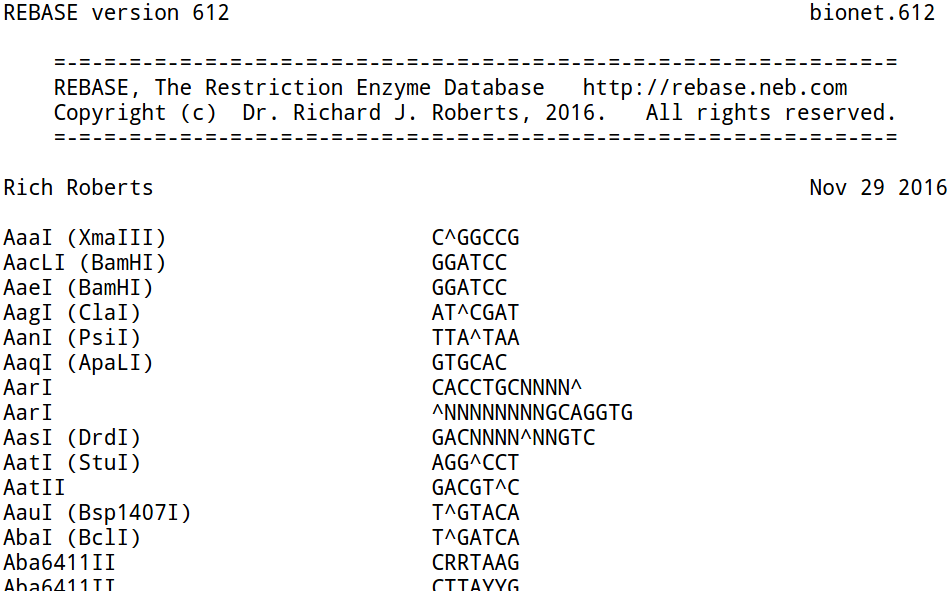
\includegraphics[width=0.9\textwidth]{c9.enzyme.rebase.bionet.file.png}
  \end{figure}
\end{frame}

\begin{frame}
  \frametitle{酶切图谱 | 限制酶数据 | 读取bionet}
  \begin{block}{任务}
    \begin{itemize}
      \item 读入bionet这个文件
      \item 获取每一个酶的名字和识别位点
      \item (简化问题)把小括号中的限制酶的名字丢掉
    \end{itemize}
  \end{block}
\end{frame}

\begin{frame}[fragile]
  \frametitle{酶切图谱 | 限制酶数据 | 读取bionet | 伪代码}
\begin{lstlisting}[basicstyle=\small\tt]
Discard header lines 

For each data line:

  remove parenthesized names, for simplicity's sake

  get and store the name and the recognition site

  Translate the recognition sites to regular expressions
    --but keep the recognition site, for printing out results
}

return the names, recognition sites, and the regular expressions
\end{lstlisting}
\end{frame}

\begin{frame}[fragile]
  \frametitle{酶切图谱 | 限制酶数据 | 读取bionet | 伪代码 | 头信息}
\begin{lstlisting}
# Discard header lines
# This keeps reading lines, up to a line containing "Rich Roberts"
foreach line 
  if /Rich Roberts/ 
    break out of the foreach loop
}
\end{lstlisting}
\end{frame}


\begin{frame}[fragile]
  \frametitle{酶切图谱 | 限制酶数据 | 读取bionet | 伪代码 | 数据信息}
\begin{lstlisting}[basicstyle=\small\tt]
For each data line:

  # Split the two or three (if there's a parenthesized name) fields
  @fields = split( " ", $_ );
  # Get and store the name and the recognition site
  $name = shift @fields;
  $site = pop @fields;

  # Translate the recognition sites to regular expressions
    --but keep the recognition site, for printing out results
}

return the names, recognition sites, and the regular expressions
\end{lstlisting}
\end{frame}

\begin{frame}[fragile]
  \frametitle{酶切图谱 | 限制酶数据 | 读取bionet | 伪代码 | \alert{补充说明}}
\begin{lstlisting}
# 提取用空白分隔的单词,保存到数组
# 处理的是存储在特殊变量$_中的行
@fields = split( " ", $_ );

# 提取数组中的第一个元素
$name = shift @fields;

# 提取数组中的最后一个元素
$site = pop @fields;
\end{lstlisting}
\end{frame}

\begin{frame}
  \frametitle{酶切图谱 | 限制酶数据 | REBASE | bionet | 文件}
  \begin{figure}
    \centering
    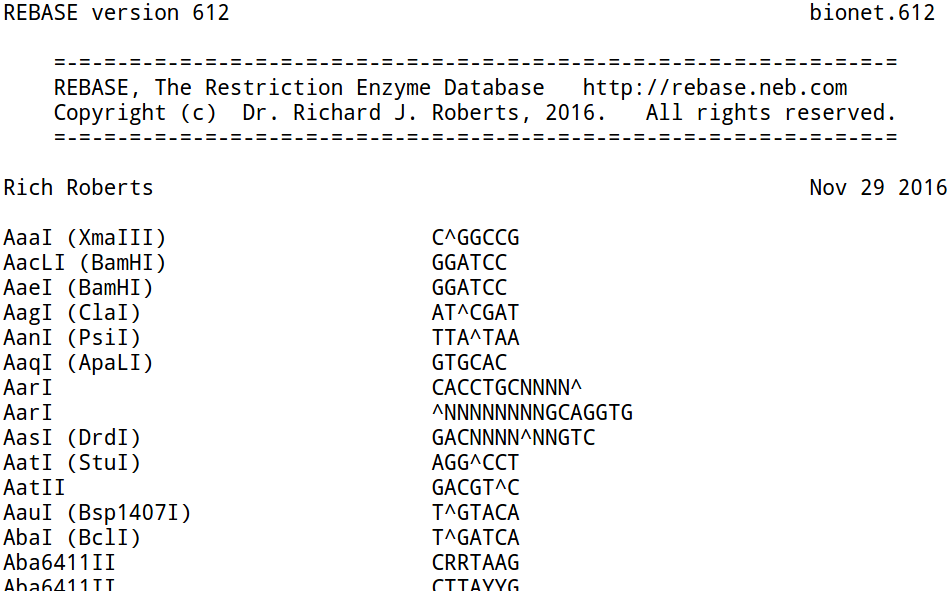
\includegraphics[width=0.9\textwidth]{c9.enzyme.rebase.bionet.file.png}
  \end{figure}
\end{frame}

\begin{frame}[fragile]
  \frametitle{酶切图谱 | 限制酶数据 | IUB2RE | 程序9.1.1}
%\begin{lstlisting}[firstnumber=1,basicstyle=\footnotesize\tt,numberstyle=\footnotesize]
\begin{lstlisting}
# Example 9-1 Translate IUB ambiguity codes to regular expressions
# IUB_to_regexp
#
# A subroutine that, given a sequence with IUB ambiguity codes,
# outputs a translation with IUB codes changed to regular expressions
\end{lstlisting}
\end{frame}

\begin{frame}[fragile]
  \frametitle{酶切图谱 | 限制酶数据 | IUB2RE | 程序9.1.2}
\begin{lstlisting}[firstnumber=7]
# These are the IUB ambiguity codes
# (Eur. J. Biochem. 150: 1-5, 1985):
# R = G or A
# Y = C or T
# M = A or C
# K = G or T
# S = G or C
# W = A or T
# B = not A (C or G or T)
# D = not C (A or G or T)
# H = not G (A or C or T)
# V = not T (A or C or G)
# N = A or C or G or T
\end{lstlisting}
\end{frame}

\begin{frame}[fragile]
  \frametitle{酶切图谱 | 限制酶数据 | IUB2RE | 程序9.1.3}
\begin{lstlisting}[firstnumber=21]
sub IUB_to_regexp {

    my ($iub) = @_;

    my $regular_expression = '';
\end{lstlisting}
\end{frame}

\begin{frame}[fragile]
  \frametitle{酶切图谱 | 限制酶数据 | IUB2RE | 程序9.1.4}
\begin{lstlisting}[firstnumber=27,basicstyle=\small\tt,numberstyle=\footnotesize]
    my %iub2character_class = (

        A => 'A',
        C => 'C',
        G => 'G',
        T => 'T',
        R => '[GA]',
        Y => '[CT]',
        M => '[AC]',
        K => '[GT]',
        S => '[GC]',
        W => '[AT]',
        B => '[CGT]',
        D => '[AGT]',
        H => '[ACT]',
        V => '[ACG]',
        N => '[ACGT]',
    );
\end{lstlisting}
\end{frame}

\begin{frame}[fragile]
  \frametitle{酶切图谱 | 限制酶数据 | IUB2RE | 程序9.1.5}
\begin{lstlisting}[firstnumber=46]
    # Remove the ^ signs from the recognition sites
    $iub =~ s/\^//g;

    # Translate each character in the iub sequence
    for ( my $i = 0 ; $i < length($iub) ; ++$i ) {
        $regular_expression .= $iub2character_class{ substr( $iub, $i, 1 ) };
    }

    return $regular_expression;
}
\end{lstlisting}
\end{frame}

\begin{frame}
  \frametitle{酶切图谱 | 限制酶数据 | 解析REBASE | 返回数据}
  \begin{block}{目标}
    对于REBASE文件的每一行,返回三个数据:酶的名字、识别位点和正则表达式
  \end{block}
  \pause
  \begin{block}{策略一}
    \begin{itemize}
      \item 使用数组:把三个数据项连续的存储在一起
      \item 读入数据:从数组中读取成组的三个项目
      \item 查询:有点困难……
    \end{itemize}
  \end{block}
  \pause
  \begin{block}{\textbf{策略二}}
    \begin{itemize}
      \item 使用散列:键为酶的名字,值为用空格分隔的识别位点和正则表达式
      \item 查询:快速
      \item 提取信息:使用split函数
    \end{itemize}
  \end{block}
\end{frame}

\begin{frame}[fragile]
  \frametitle{酶切图谱 | 限制酶数据 | 解析REBASE | 程序9.2.1}
\begin{lstlisting}[firstnumber=1]
# Example 9-2 Subroutine to parse a REBASE datafile
# parseREBASE-Parse REBASE bionet file
#
# A subroutine to return a hash where
#    key   = restriction enzyme name
#    value = whitespace-separated recognition site and regular expression
\end{lstlisting}
\end{frame}

\begin{frame}[fragile]
  \frametitle{酶切图谱 | 限制酶数据 | 解析REBASE | 程序9.2.2}
\begin{lstlisting}[firstnumber=8]
sub parseREBASE {

    my ($rebasefile) = @_;

    use strict;
    use warnings;
    use BeginPerlBioinfo;    # see Chapter 6 about this module

    # Declare variables
    my @rebasefile  = ();
    my %rebase_hash = ();
    my $name;
    my $site;
    my $regexp;
\end{lstlisting}
\end{frame}

\begin{frame}[fragile]
  \frametitle{酶切图谱 | 限制酶数据 | 解析REBASE | 程序9.2.3}
\begin{lstlisting}[firstnumber=23,basicstyle=\small\tt,numberstyle=\footnotesize]
    # Read in the REBASE file
    my $rebase_filehandle = open_file($rebasefile);

    while (<$rebase_filehandle>) {

        # Discard header lines
        ( 1 .. /Rich Roberts/ ) and next;

        # Discard blank lines
        /^\s*$/ and next;

        # Split the two (or three if includes parenthesized name) fields
        my @fields = split( " ", $_ );

        # Get and store the name and the recognition site
\end{lstlisting}
\end{frame}

\begin{frame}[fragile]
  \frametitle{酶切图谱 | 限制酶数据 | 解析REBASE | 程序9.2.4}
\begin{lstlisting}[firstnumber=37,basicstyle=\footnotesize\tt,numberstyle=\scriptsize]
        # Remove parenthesized names, for simplicity's sake,
        # by not saving the middle field, if any,
        # just the first and last
        $name = shift @fields;

        $site = pop @fields;

        # Translate the recognition sites to regular expressions
        $regexp = IUB_to_regexp($site);

        # Store the data into the hash
        $rebase_hash{$name} = "$site $regexp";
    }

    # Return the hash containing the reformatted REBASE data
    return %rebase_hash;
}
\end{lstlisting}
\end{frame}

\subsection{操作符}
\begin{frame}[fragile]
  \frametitle{酶切图谱 | 限制酶数据 | 解析REBASE | 程序9.2 | \alert{范围操作符}}
\begin{lstlisting}
( 1 .. /Rich Roberts/ ) and next;
\end{lstlisting}
\pause
\begin{block}{说明}
  \begin{itemize}
    \item \verb|..|:范围操作符(range operator)
    \item 跳过头信息(从第一行到包含“Rich Roberts”的行)
    \item and:逻辑操作符
  \end{itemize}
\end{block}
\end{frame}

\begin{frame}[fragile]
  \frametitle{酶切图谱 | 限制酶数据 | 解析REBASE | 程序9.2 | \alert{逻辑操作符}}
  \begin{block}{逻辑操作符(logical operator)}
    \begin{itemize}
      \item and:测试两个条件是不是都为真
      \item or:测试是不是至少有一个条件为真
      \item not:否定操作符,测试某个条件是不是为假
    \end{itemize}
  \end{block}
  \pause
  \begin{block}{补充说明}
    \begin{itemize}
      \item 与and、or和not相关的操作符分别是 \verb|&&|、\verb=||=和 \verb|!|;它们的优先级不同
      \item 对优先级不确定时,用小括号把表达式包裹起来,确保语句的执行结果和预期一样
    \end{itemize}
  \end{block}
\end{frame}

\begin{frame}[fragile]
  \frametitle{酶切图谱 | 限制酶数据 | 解析REBASE | 程序9.2 | \alert{逻辑操作符}}
\begin{lstlisting}
# and:只有当两个条件都为真时,整个语句才为真
if( $string eq 'kinase' and $num == 3 ) {
  ...
}

# or:如果两个条件中至少有一个为真,整个语句就为真
if( $string eq 'kinase' or $num == 3 ) {
  ...
}

# not:条件为假,被not否定后,整个语句为真
if( not 6 == 9 ) {
  ...
}
\end{lstlisting}
\end{frame}

\begin{frame}[fragile]
  \frametitle{酶切图谱 | 限制酶数据 | 解析REBASE | 程序9.2 | \alert{逻辑操作符}}
  \begin{block}{and的求值顺序:类似if语句}
    \begin{itemize}
      \item 首先对左边的参数进行求值
	\begin{itemize}
	  \item 如果左边为真,对右边的参数求值并返回结果
	  \item 如果左边为假,右边的参数永远不会被求值
	\end{itemize}
    \end{itemize}
  \end{block}
  \pause
\begin{lstlisting}
if( $verbose  ) {
  print $helpful_but_verbose_message;
}

$verbose and print $helpful_but_verbose_message;
\end{lstlisting}
\end{frame}

\begin{frame}[fragile]
  \frametitle{酶切图谱 | 限制酶数据 | 解析REBASE | 程序9.2 | \alert{逻辑操作符}}
  \begin{block}{or的求值顺序}
    \begin{itemize}
      \item 首先对左边的参数进行求值
	\begin{itemize}
	  \item 如果左边为真,就直接返回结果
	  \item 如果左边为假,对右边的参数求值并返回结果
	\end{itemize}
    \end{itemize}
  \end{block}
  \pause
\begin{lstlisting}
unless(open(MYFILE, $file)) {
  print "I cannot open file $file\n";
  exit;
}

open(MYFILE, $file) or die "I cannot open file $file: $!";
\end{lstlisting}
\end{frame}

\begin{frame}[fragile]
  \frametitle{酶切图谱 | 限制酶数据 | 解析REBASE | 程序9.2 | 说明}
\begin{lstlisting}
# 跳过头部的信息行
( 1 .. /Rich Roberts/ ) and next;

# 跳过空白行
/^\s*$/ and next;
\end{lstlisting}
\end{frame}

\subsection{制作酶切图谱}
\begin{frame}[fragile]
  \frametitle{酶切图谱 | 制作图谱 | 伪代码}
\begin{lstlisting}
# Get DNA
get_file_data

extract_sequence_from_fasta_data

# Get the REBASE data into a hash, from file "bionet"
parseREBASE('bionet');

for each user query

  If query is defined in the hash
    Get positions of query in DNA

  Report on positions, if any
}
\end{lstlisting}
\end{frame}

\begin{frame}[fragile]
  \frametitle{酶切图谱 | 制作图谱 | 伪代码 | 子程序}
  \begin{block}{子程序}
    \begin{itemize}
      \item 已有:extract\_sequence\_from\_fasta\_data
      \item 尚缺:在DNA中查询并返回匹配的位置
    \end{itemize}
  \end{block}
  \pause
\begin{lstlisting}
Given arguments $query and $dna

while ( $dna =~ /$query/ig ) {
  save the position of the match
}

return @positions
\end{lstlisting}
\end{frame}

\begin{frame}[fragile]
  \frametitle{酶切图谱 | 制作图谱 | 伪代码 | \alert{子程序}}
\begin{lstlisting}[basicstyle=\small\tt,numberstyle=\footnotesize]
# Find locations of a match of a regular expression in a string
# return an array of positions where the regular expression appears in the string
sub match_positions {
    my ( $regexp, $sequence ) = @_;
    use strict;
    use BeginPerlBioinfo;
    # Declare variables
    my @positions = ();
    # Determine positions of regular expression matches
    while ( $sequence =~ /$regexp/ig ) {
        push( @positions, pos($sequence) - length($&) + 1 );
    }
    return @positions;
}
\end{lstlisting}
\end{frame}

\begin{frame}[fragile]
  \frametitle{酶切图谱 | 制作图谱 | 伪代码 | 子程序 | 说明 | \alert{特殊变量}}
  \begin{block}{特殊变量}
    \begin{itemize}
      \item \verb|$&|:字符串中实际匹配模式的部分
      \item \verb|$`|:字符串中匹配模式前面的所有内容
      \item \verb|$'|:字符串中匹配模式后面的所有内容
    \end{itemize}
  \end{block}
  \pause
\begin{lstlisting}
my $string = "abcdef";
while ( $string =~ /cd/g ) {
    print "Prematch: $`\n";
    print "Match: $&\n";
    print "Posmatch: $'\n";
}
# $`:ab; $&:cd; $':ef
\end{lstlisting}
\end{frame}

\begin{frame}[fragile]
  \frametitle{酶切图谱 | 制作图谱 | 伪代码 | 子程序 | 说明 | \alert{pos}}
  \begin{block}{pos}
    \begin{itemize}
      \item pos:返回匹配序列后面第一个字符的索引位置
      \item pos - length:匹配序列第一个字符的索引位置
    \end{itemize}
  \end{block}
  \pause
\begin{lstlisting}[basicstyle=\small\tt,numberstyle=\footnotesize]
my $string = "abcdef";
# 0-index: 0 1 2 3 4 5
# string : a b c d e f
# 1-index: 1 2 3 4 5 6
while ( $string =~ /cd/g ) {
    my $pos    = pos($string);
    my $start0 = $pos - length($&);
    my $start1 = $pos - length($&) + 1;
    print "Number for pos(function): $pos\n";
    print "Number for start(0-index): $start0\n";
    print "Number for start(1-index): $start1\n";
}
# 4 2 3
\end{lstlisting}
\end{frame}

\begin{frame}[fragile]
  \frametitle{酶切图谱 | 制作图谱 | 程序9.3.1}
\begin{lstlisting}[firstnumber=1,basicstyle=\small\tt,numberstyle=\footnotesize]
#!/usr/bin/perl -w
# Example 9-3   Make restriction map from user queries on names of restriction enzymes

use strict;
use warnings;
use BeginPerlBioinfo;    # see Chapter 6 about this module

# Declare and initialize variables
my %rebase_hash      = ();
my @file_data        = ();
my $query            = '';
my $dna              = '';
my $recognition_site = '';
my $regexp           = '';
my @locations        = ();
\end{lstlisting}
\end{frame}

\begin{frame}[fragile]
  \frametitle{酶切图谱 | 制作图谱 | 程序9.3.2}
\begin{lstlisting}[firstnumber=17]
# Read in the file "sample.dna"
@file_data = get_file_data("sample.dna");

# Extract the DNA sequence data from the contents of the file "sample.dna"
$dna = extract_sequence_from_fasta_data(@file_data);

# Get the REBASE data into a hash, from file "bionet"
%rebase_hash = parseREBASE('bionet');

# Prompt user for restriction enzyme names, create restriction map
\end{lstlisting}
\end{frame}

\begin{frame}[fragile]
  \frametitle{酶切图谱 | 制作图谱 | 程序9.3.3}
\begin{lstlisting}[firstnumber=27]
do {
    print "Search for what restriction site for (or quit)?: ";

    $query = <STDIN>;

    chomp $query;

    # Exit if empty query
    if ( $query =~ /^\s*$/ ) {

        exit;
    }
\end{lstlisting}
\end{frame}

\begin{frame}[fragile]
  \frametitle{酶切图谱 | 制作图谱 | 程序9.3.4}
\begin{lstlisting}[firstnumber=40]
    # Perform the search in the DNA sequence
    if ( exists $rebase_hash{$query} ) {

        ( $recognition_site, $regexp ) = split( " ", $rebase_hash{$query} );

        # Create the restriction map
        @locations = match_positions( $regexp, $dna );
\end{lstlisting}
\end{frame}

\begin{frame}[fragile]
  \frametitle{酶切图谱 | 制作图谱 | 程序9.3.5}
\begin{lstlisting}[firstnumber=48,basicstyle=\small\tt,numberstyle=\footnotesize]
        # Report the restriction map to the user
        if (@locations) {
            print "Searching for $query $recognition_site $regexp\n";
            print "A restriction site for $query at locations:\n";
            print join( " ", @locations ), "\n";
        }
        else {
            print "A restriction enzyme $query is not in the DNA:\n";
        }
    }
    print "\n";
} until ( $query =~ /quit/ );

exit;
\end{lstlisting}
\end{frame}

\begin{frame}[fragile]
  \frametitle{酶切图谱 | 制作图谱 | 程序9.3 | 输出}
\begin{lstlisting}[basicstyle=\footnotesize\tt,numberstyle=\scriptsize]
Search for what restriction enzyme (or quit)?: AceI
Searching for AceI G^CWGC GC[AT]GC
A restriction site for AceI at locations:
54 94 582 660 696 702 840 855 957

Search for what restriction enzyme (or quit)?: AccII
Searching for AccII CG^CG CGCG
A restriction site for AccII at locations:
181

Search for what restriction enzyme (or quit)?: AaeI
A restriction site for AaeI is not in the DNA:

Search for what restriction enzyme (or quit)?: quit
\end{lstlisting}
\end{frame}

\section{操作符优先级}
\begin{frame}
  \frametitle{酶切图谱 | 优先级 | 简介}
  \begin{block}{优先级(precedence)}
    在数学和计算机科学中,运算次序(也称为运算顺序、运算子优先级)是指决定在表示式中的哪一运算子首先被执行的规则。\\
    \vspace{1em}
    比如,在四则运算中,一般有先乘除后加减的规定。就是说在 $2 + 3 \times 4 $ 这样的式子中,按规定会先对3和4作乘法,得出12,然后再把2和12加起来,最后就得出14。
  \end{block}
\end{frame}

\begin{frame}
  \frametitle{酶切图谱 | 优先级 | 规定}
  \begin{figure}
    \centering
    \includegraphics[width=0.8\textwidth]{c9.enzyme.perl.precedence.01.png}
  \end{figure}
\end{frame}

\begin{frame}
  \frametitle{酶切图谱 | 优先级 | 规定}
  \begin{figure}
    \centering
    \includegraphics[width=0.8\textwidth]{c9.enzyme.perl.precedence.02.png}
  \end{figure}
\end{frame}

\begin{frame}
  \frametitle{酶切图谱 | 优先级 | 原则}
  \begin{block}{实例}
    \begin{itemize}
      \item $10 + 8 / 4 - 2 \times 3 = 10$
      \item $10 + (8 / 4) - (2 \times 3) = 6$
      \item $10 + (8 / 4 - 2) \times 3 = 10$
    \end{itemize}
  \end{block}
  \pause
  \begin{block}{\alert{基本原则}}
    \begin{itemize}
      \item (在复杂的表达式中)使用括号明确优先级
      \item 好处:不用背/查优先级表,避免大量的程序调试,……
    \end{itemize}
  \end{block}
\end{frame}

\section{回顾和总结}
\subsection{总结}
\begin{frame}
  \frametitle{酶切图谱 | 总结}
  \begin{block}{知识点}
    \begin{itemize}
      \item 正则表达式基础:基本概念、基础理论、基本语法
      \item 正则表达式应用:元字符,解析,构建
      \item 操作符:范围操作符,逻辑操作符,优先级
      \item 逻辑操作符:求值顺序,应用
      \item 模式匹配:特殊变量,pos函数
    \end{itemize}
  \end{block}
  \pause
  \begin{block}{技能}
    \begin{itemize}
      \item 能够把IUB代码翻译成正则表达式
      \item 能够编写制作酶切图谱相关的Perl程序
    \end{itemize}
  \end{block}
\end{frame}

\subsection{思考题}
\begin{frame}
  \frametitle{酶切图谱 | 思考题}
  \begin{enumerate}
    \item 总结正则表达式的基本运算。
    \item 总结正则表达式的基本语法。
    \item 举例说明正则表达式中的元字符。
    \item 解析正则表达式实例。
    \item 根据要求编写正则表达式。
    \item 举例说明范围操作符的使用。
    \item 列举常见的逻辑操作符,并解释其求值顺序。
    \item 列举模式匹配中的特殊变量,举例进行说明。
    \item 如何明确复杂表达式中操作的优先级?
  \end{enumerate}
\end{frame}


\input{snippet/class_tail.tex}
